\documentclass[11pt,a4paper]{article}

\usepackage[margin=2.2cm]{geometry}
\usepackage[T1]{fontenc}
\usepackage{lmodern}
\usepackage{microtype}
\usepackage{parskip}
\usepackage{titlesec}
\usepackage{titling}
\usepackage{booktabs}
\usepackage{tabularx}
\usepackage{array}
\usepackage{xcolor}
\usepackage{tikz}
\usepackage{pgf}
\usetikzlibrary{arrows.meta, positioning, fit, backgrounds, shapes.geometric}
\usepackage{enumitem}
\usepackage{hyperref}
\usepackage{fancyhdr}
\usepackage{mdframed}

% ── Colours ────────────────────────────────────────────────────────────────────
\definecolor{primary}{HTML}{1A1A2E}
\definecolor{accent}{HTML}{0F3460}
\definecolor{highlight}{HTML}{E94560}
\definecolor{lightgray}{HTML}{F5F5F5}
\definecolor{midgray}{HTML}{CCCCCC}
\definecolor{darkgray}{HTML}{555555}

% ── Section headings ───────────────────────────────────────────────────────────
\titleformat{\section}{\large\bfseries\color{accent}}{}{0em}{}[\color{midgray}\titlerule]
\titleformat{\subsection}{\normalsize\bfseries\color{primary}}{}{0em}{}
\titlespacing{\section}{0pt}{18pt}{6pt}
\titlespacing{\subsection}{0pt}{10pt}{3pt}

% ── Header / footer ────────────────────────────────────────────────────────────
\pagestyle{fancy}
\fancyhf{}
\renewcommand{\headrulewidth}{0.4pt}
\fancyhead[L]{\small\color{darkgray}Kamka CloudOps Platform — Technical Report}
\fancyhead[R]{\small\color{darkgray}Omar Chouchane}
\fancyfoot[C]{\small\color{darkgray}\thepage}

% ── Hyperlinks ─────────────────────────────────────────────────────────────────
\hypersetup{colorlinks=true, linkcolor=accent, urlcolor=accent}

% ── Helpers ────────────────────────────────────────────────────────────────────
\newcommand{\tech}[1]{\textbf{#1}}
\newcolumntype{L}{>{\raggedright\arraybackslash}X}

% ───────────────────────────────────────────────────────────────────────────────
\begin{document}

% ── Title block ────────────────────────────────────────────────────────────────
\begin{center}
  {\LARGE\bfseries\color{primary} Kamka CloudOps Platform}\\[4pt]
  {\large\color{darkgray} Technical Report}\\[8pt]
  {\small\color{darkgray} Omar Chouchane \quad|\quad DevOps Engineering Assessment \quad|\quad June 2026}
\end{center}

\vspace{4pt}
\noindent\color{midgray}\rule{\linewidth}{0.6pt}
\vspace{6pt}

% ── 1. Architecture ────────────────────────────────────────────────────────────
\section{Architecture}

\subsection{Services}

The platform runs as a set of Docker containers managed by Compose on a single AWS EC2 instance. All traffic enters through Caddy, which terminates HTTP and proxies to the application tier.

\vspace{10pt}
\begin{center}
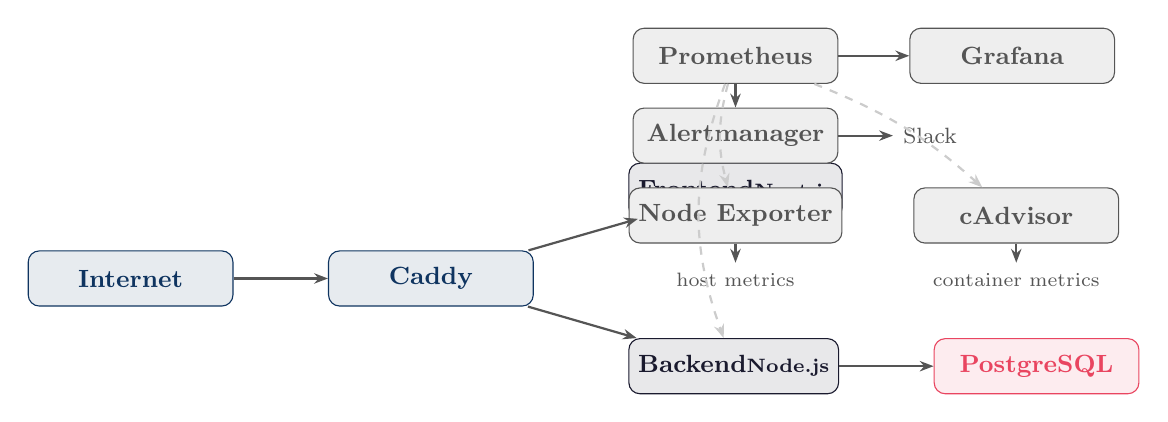
\begin{tikzpicture}[
  box/.style={rectangle, rounded corners=4pt, draw=#1, fill=#1!10,
              minimum width=2.6cm, minimum height=0.7cm,
              font=\small\bfseries, text=#1},
  arr/.style={-{Stealth[length=5pt]}, thick, color=darkgray},
  lbl/.style={font=\footnotesize\color{darkgray}},
  node distance=0.5cm and 1.1cm
]

% Internet
\node[box=accent] (internet) {Internet};

% Caddy
\node[box=accent, right=1.2cm of internet] (caddy) {Caddy};

% App tier
\node[box=primary, above right=0.4cm and 1.2cm of caddy] (frontend) {Frontend\\[-2pt]\scriptsize Next.js};
\node[box=primary, below right=0.4cm and 1.2cm of caddy] (api) {Backend\\[-2pt]\scriptsize Node.js};

% DB
\node[box=highlight, right=1.2cm of api] (postgres) {PostgreSQL};

% Observability
\node[box=darkgray, above=1.0cm of frontend] (prometheus) {Prometheus};
\node[box=darkgray, right=0.9cm of prometheus] (grafana) {Grafana};
\node[box=darkgray, below=0.3cm of prometheus] (alertmanager) {Alertmanager};
\node[box=darkgray, below=0.3cm of alertmanager] (nodeexp) {Node Exporter};
\node[box=darkgray, right=0.9cm of nodeexp] (cadvisor) {cAdvisor};

% Arrows
\draw[arr] (internet) -- (caddy);
\draw[arr] (caddy) -- (frontend);
\draw[arr] (caddy) -- (api);
\draw[arr] (api) -- (postgres);
\draw[arr] (prometheus) -- (alertmanager);
\draw[arr] (alertmanager) -- ++(2,0) node[lbl, anchor=west]{Slack};
\draw[arr] (prometheus) -- (grafana);
\draw[arr] (nodeexp) -- ++(0,-0.6) node[lbl, anchor=north]{\scriptsize host metrics};
\draw[arr] (cadvisor) -- ++(0,-0.6) node[lbl, anchor=north]{\scriptsize container metrics};

% Scrape arrows (dashed)
\draw[arr, dashed, color=midgray] (prometheus) to[bend right=15] (nodeexp);
\draw[arr, dashed, color=midgray] (prometheus) to[bend left=10] (cadvisor);
\draw[arr, dashed, color=midgray] (prometheus) to[bend right=20] (api);

\end{tikzpicture}
\end{center}

\subsection{CI/CD Pipeline — Change Flow}

A push to \texttt{master} triggers the following sequential pipeline. Jobs 1 and 2 run in parallel; Job 3 requires both.

\vspace{10pt}
\begin{center}
\begin{tikzpicture}[
  job/.style={rectangle, rounded corners=3pt, draw=accent, fill=accent!8,
              minimum width=3.2cm, minimum height=1.4cm,
              align=center, font=\small},
  step/.style={font=\scriptsize\color{darkgray}, align=center},
  arr/.style={-{Stealth[length=5pt]}, thick, color=accent},
  node distance=0.6cm and 0.5cm
]

\node[job] (j1) {\textbf{1 · Lint \& Test}\\[3pt]
  \step{ESLint · Prettier\\Mocha integration tests}};

\node[job, below=0.5cm of j1] (j2) {\textbf{2 · Security Scan}\\[3pt]
  \step{SonarCloud SAST\\Trivy FS scan → Slack}};

\node[job, right=2.2cm of j1, yshift=-0.9cm] (j3) {\textbf{3 · Build \& Push}\\[3pt]
  \step{Docker build\\Trivy image scan → Slack\\Push to GHCR}};

\node[job, right=2.0cm of j3] (j4) {\textbf{4 · Deploy}\\[3pt]
  \step{SSH to EC2\\Rolling update\\DB migrate · health check\\Slack notify}};

\draw[arr] (j1.east) -- (j3.west|-j1.east) -- (j3.west);
\draw[arr] (j2.east) -- (j3.west|-j2.east) -- (j3.west);
\draw[arr] (j3) -- (j4);

\node[step, above=0.15cm of j1]{\textit{git push → master}};

% OIDC note
\node[step, below=0.15cm of j4, text=highlight]{\small OIDC — no static AWS keys};

\end{tikzpicture}
\end{center}

\vspace{4pt}
A change goes from \texttt{git push} to running in production in under 5 minutes. The deploy job uses a rolling update (one service at a time) and exits non-zero if the health check fails, which halts the pipeline.

% ── 2. Key Decisions ───────────────────────────────────────────────────────────
\section{Key Decisions and Trade-offs}

\begin{tabularx}{\linewidth}{@{}lLL@{}}
\toprule
\textbf{Decision} & \textbf{Choice \& Reason} & \textbf{Trade-off} \\
\midrule
\textbf{Registry} &
  GHCR. Free for public repos, integrated with GitHub Actions via \texttt{GITHUB\_TOKEN} — no separate registry to manage. &
  Tied to GitHub. A move to GitLab or self-hosted would require a registry migration. \\
\addlinespace
\textbf{Secrets} &
  AWS SSM Parameter Store (SecureString). Secrets are fetched at deploy time, never written to disk or env files. The server and GitHub Actions each have a separate, least-privilege IAM role. &
  Requires AWS CLI on the server at startup. Rotating a secret means re-running the deploy. \\
\addlinespace
\textbf{Auth (CI → AWS)} &
  GitHub Actions OIDC. The pipeline assumes an IAM role via a short-lived token — no long-lived access keys exist anywhere. &
  OIDC provider and trust policy must be maintained in Terraform. First-time setup is more complex than a static key. \\
\addlinespace
\textbf{Monitoring} &
  Prometheus + Grafana + Alertmanager. Open-source, self-hosted, and composable. Six alert rules cover CPU, memory, disk, containers, error rate, and backup freshness. &
  Self-hosted means we maintain the stack. A managed service (Datadog, Grafana Cloud) would reduce ops burden at higher cost. \\
\addlinespace
\textbf{Dev/prod parity} &
  Both environments use Docker Compose with identical images. Dev uses \texttt{docker-compose.dev.yml} (nodemon, hot-reload). Prod uses \texttt{docker-compose.prod.yml} (read-only FS, non-root user, resource limits). Differences are explicit and minimal. &
  Single-node prod means no horizontal scaling. A Kubernetes-based approach would give better parity with a scaled production environment. \\
\addlinespace
\textbf{Reverse proxy} &
  Caddy. Automatic HTTPS via Let's Encrypt with a one-line config. Proxies \texttt{/api}, \texttt{/healthz}, \texttt{/grafana}, and all other paths to the correct upstream. &
  Less flexible than Nginx for advanced routing. Caddy's plugin ecosystem is smaller. \\
\bottomrule
\end{tabularx}

% ── 3. Known Limitations ───────────────────────────────────────────────────────
\section{Known Limitations and What I Would Do With More Time}

\begin{itemize}[leftmargin=*, itemsep=4pt]

  \item \textbf{Single EC2 node.} The entire stack — app, database, and observability — runs on one \texttt{t3.micro}. A failure of that instance takes everything down. With more time: move PostgreSQL to RDS (managed failover), put the app tier behind an ALB, and use an Auto Scaling Group.

  \item \textbf{No container orchestration.} Docker Compose does not reschedule failed containers across nodes. Migration to ECS Fargate or Kubernetes (EKS) would give proper scheduling, rolling deployments, and horizontal scaling without manual intervention.

  \item \textbf{Backup untested end-to-end.} \texttt{backup.sh} writes to S3 and records a Prometheus metric, but a restore procedure has not been tested. Backups without verified restores are not backups.

  \item \textbf{Alertmanager channel override.} Alertmanager's Slack receiver does not support overriding the webhook's default channel in the payload (Slack rejects the request). The alert message goes to whichever channel the webhook was created for. A proper fix is to provision a Slack app with \texttt{chat:write} scope instead of an incoming webhook.

  \item \textbf{Observability gaps.} Prometheus scrapes Node Exporter, cAdvisor, and the API's \texttt{/metrics} endpoint. The frontend has no instrumentation. Distributed tracing (OpenTelemetry) and structured logging aggregation (Loki) are absent.

  \item \textbf{Secrets rotation.} Updating a secret in SSM requires re-running the deploy to pick up the new value. An agent like AWS Secrets Manager with automatic rotation and dynamic injection would remove this manual step.

  \item \textbf{SSH-based deploy.} The deploy job SSHes into the instance and runs commands directly. This is simple but fragile — a connection drop mid-deploy can leave the stack in an inconsistent state. A proper solution uses a deploy agent (SSM Run Command, or a CD tool like ArgoCD) with rollback built in.

\end{itemize}

\vspace{12pt}
\noindent\color{midgray}\rule{\linewidth}{0.4pt}
\vspace{4pt}
\begin{center}
  \small\color{darkgray}
  Repository: \href{https://github.com/OmarChouchane/kamka-cloudops-platform}{github.com/OmarChouchane/kamka-cloudops-platform}
\end{center}

\end{document}
